%/*% pdflatex -file-line-error -interaction nonstopmode %

\documentclass{article}
\usepackage{graphicx}
\graphicspath{ {./imagescopy/standard_test/} }
\usepackage{amsmath}
\usepackage{amsfonts}
\usepackage{bookmark}
\usepackage{exercises}
\usepackage{amsthm}
\usepackage{yhmath}
\usepackage{placeins}
\newcommand*{\oldneg}{\mathord{\sim}}

\theoremstyle{definition}
\newtheorem{definition}{Definition}

\setlength{\parindent}{.5in}
\setlength{\parskip}{12pt}

\title{Stand Test Practice}
\begin{document}
\maketitle

\section*{1}
B

\section*{2}
B

\section*{3}
B

\section*{4}
C

\section*{5}
B

\section*{6}
B

\section*{7}
B

\section*{8}
D

\section*{9}
We are give that $6x^2-11x-10=(3x+2)(2x-k)\newline$ With this information, we know that $(3x+2)(2x-k)$ is a factored form of $6x^2-11x-10$. Well, 
this means that $2\times -k=-10$, and hence, $k=5$

\section*{10}
First, the standard form of $(5+i)(10-i)$ is:\newline 
$50+10i-5i-i^2=51+5i\newline$ In the above standard form, the real part is $51$.

\section*{11}
To be a perfect square trinomial, $a$ must be a perfect square and $c$ muwst be a perfect square. Also, $\sqrt{c}2\sqrt{a}$ must equal $b$, that is, 
$\sqrt{c}2(1)=7\newline\rightarrow 
\sqrt{c}=3.5\newline\rightarrow 
c=12.25$, which would make the standarad form equation turn into the factored form of $x^2-7x+12.25$ into $(x-3.5)^2$

\section*{12}
The maximum value of the function is given by the $y$-coordinate of the vertex. Becauase this equation is in vertex form, the vertex is 
$(2,6)$, meaning the maximum value of the function is $6$.

\section*{13}
To find the greatest zero of the given function, we need to solve the equation, which can be done by factoring:\newline
$x^2-25x+66=0\newline\rightarrow 
(x-22)(x-3)=0\newline\rightarrow 
x=22\vee x=3\newline$ meaning the greatest zero of the given function is $22$.

\section*{14}
The absolute value of a complex number $a+bi$ is given by $\sqrt{a^2+b^2}$, meaning the absolute value of $-5+12i$ is $\sqrt{(-5)^2+12^2}=\sqrt{169}=13$

\section*{15}
We are given that the parabola passes through the point $(0,-22)$. Because this has a $y$-coordinate of $0$, we know that this is the $y$-intercept 
of the parabola. We also know that the $y$-intercept of any parabola written in standard form is has a $y$-coordinate equal to $c$ in the standard 
form equation, meaning $c=-22$. We are also given two other points of the parabola, $(2,-6)$ and $(5,-12)$. This allows us to write the following 
two equations:
\[
\begin{array}{rl}
            & -6=a(2)^2+b(2)-22 \\
	    & -12=a(5)^2+b(5)-22
\end{array}
\] 
We can solve these systems of equations, first by solving for $b$ in equation one:
\[
\begin{array}{rl}
            & -12=a(5)^2+b(5)-22 \\
\rightarrow & -12=25a+5b-22 \\
\rightarrow & 10=25a+5b \\
\rightarrow & 10-25a=5b \\
\rightarrow & b=2-5a
\end{array}
\] 
We can then plug in this value of $b$ into the second equation, which will yield the value of $a$:
\[
\begin{array}{rl}
            & -6=a(2)^2+b(2)-22 \\
\rightarrow & 16=4a+2b \\
\rightarrow & 16=4a+2(2-5a) \\
\rightarrow & 16=4a+4-10a \\
\rightarrow & -6a=12 \\
\rightarrow & a=-2
\end{array}
\] 
Then, recalling that we have shown $b=2-5(a)$, we know that $b=2-5(-2)=12$. Because the $x$-coordinate of the vertex is given by $-\frac{b}{2a}$, we know 
that the $x$-coordinate of the vertex is $-\frac{12}{2(-2)}=3$.
\section*{16}
The minimum value of a function is given by finding the $y$-coordinate of the vertex, where $a$ is positive. The $x$-coordinate of the vertex of a standard 
form equation is given by $-\frac{b}{2a}=-\frac{24}{2(4)}=-3$, meaning the $y$-coordinate of the vertex is $4(-3)^2+24(-3)+39=3$, which is also 
the minimum value.

\section*{17}
$3x^2+6x+14=0$ (Write down given equation)
$\newline\rightarrow 3x^2+6x=-14$ (Isolate $c$ on the right hand side)
$\newline\rightarrow 3(x^2+2x)=-14$ (Factor out $3$ from $a$, in order to make $a=1$)
$\newline\rightarrow 3(x^2+2x+1)=-14+1(3)$ (Add $(\frac{b}{2})^2$ to both sides. Because a factor of $3$ has been taken out of $b$, we must also multiply 
this number by $3$)
$\newline\rightarrow 3(x+1)^2=-11$ (Factor $x^2+2x+1$ using the perfect square trinomial pattern)
$\newline\rightarrow (x+1)^2=-\frac{11}{3}$ (Divide each side by $3$)
$\newline\rightarrow x+1=\pm\sqrt{-\frac{11}{3}}$ (Take the square root of each side) 
$\newline\rightarrow x=-1\pm\frac{\sqrt{11}}{\sqrt{3}}i$ (Add $-1$ to both sides, factor out $i$ from the negative square root, and then use the rule that 
$\sqrt{\frac{a}{b}}=\frac{\sqrt{a}}{\sqrt{b}}$
$\newline\rightarrow x=-1\pm\frac{\sqrt{33}}{3}i$ (Rationalize the denominator)

\section*{18}
The graph of $y=6x^2$ moves upwards, in a similar manner to the graph of $y=x^2$. However, the graph of $6x^2$ is also much narrower than the graph of 
$x^2$.

\section*{19}
The general function for a dropped object is $h=-16t^2+t+h_0$, with all variables having the same values as in the equation given in this problem. 
The relation between this 
function and the function given in this problem is that the general function does not account for vertical velocity, or rather, it assumes a velocity
of $1$, while the function given in this problem can be obtained by taking the general function and then multiplying $t$ by the velocity, in order to 
account for a velocity of zero.

\section*{20}
To find the two points where the given graphs intersect, we need to set their $y$-coordinates equal to eachother, as the two graphs having the same 
points at a given $x$ coordinate guarantees them having the same $y$-cooridnate. Hence, we write:\newline
$2x^2-5x-12=\frac{1}{2}x^2-3x+4\newline\rightarrow 
\frac{3}{2}x^2-2x-16=0\newline\rightarrow 
x=\frac{2\pm\sqrt{(-2)^2-4(\frac{3}{2})(-16)}}{2(\frac{3}{2})}\newline\rightarrow 
x=\frac{2\pm 10}{3}\newline\rightarrow 
x=4\vee x=-\frac{8}{3}$
meaning the intersections of the graph are $(4,0)$ and $(-\frac{8}{3},\frac{140}{9})$

\section*{21}
(a): \newline 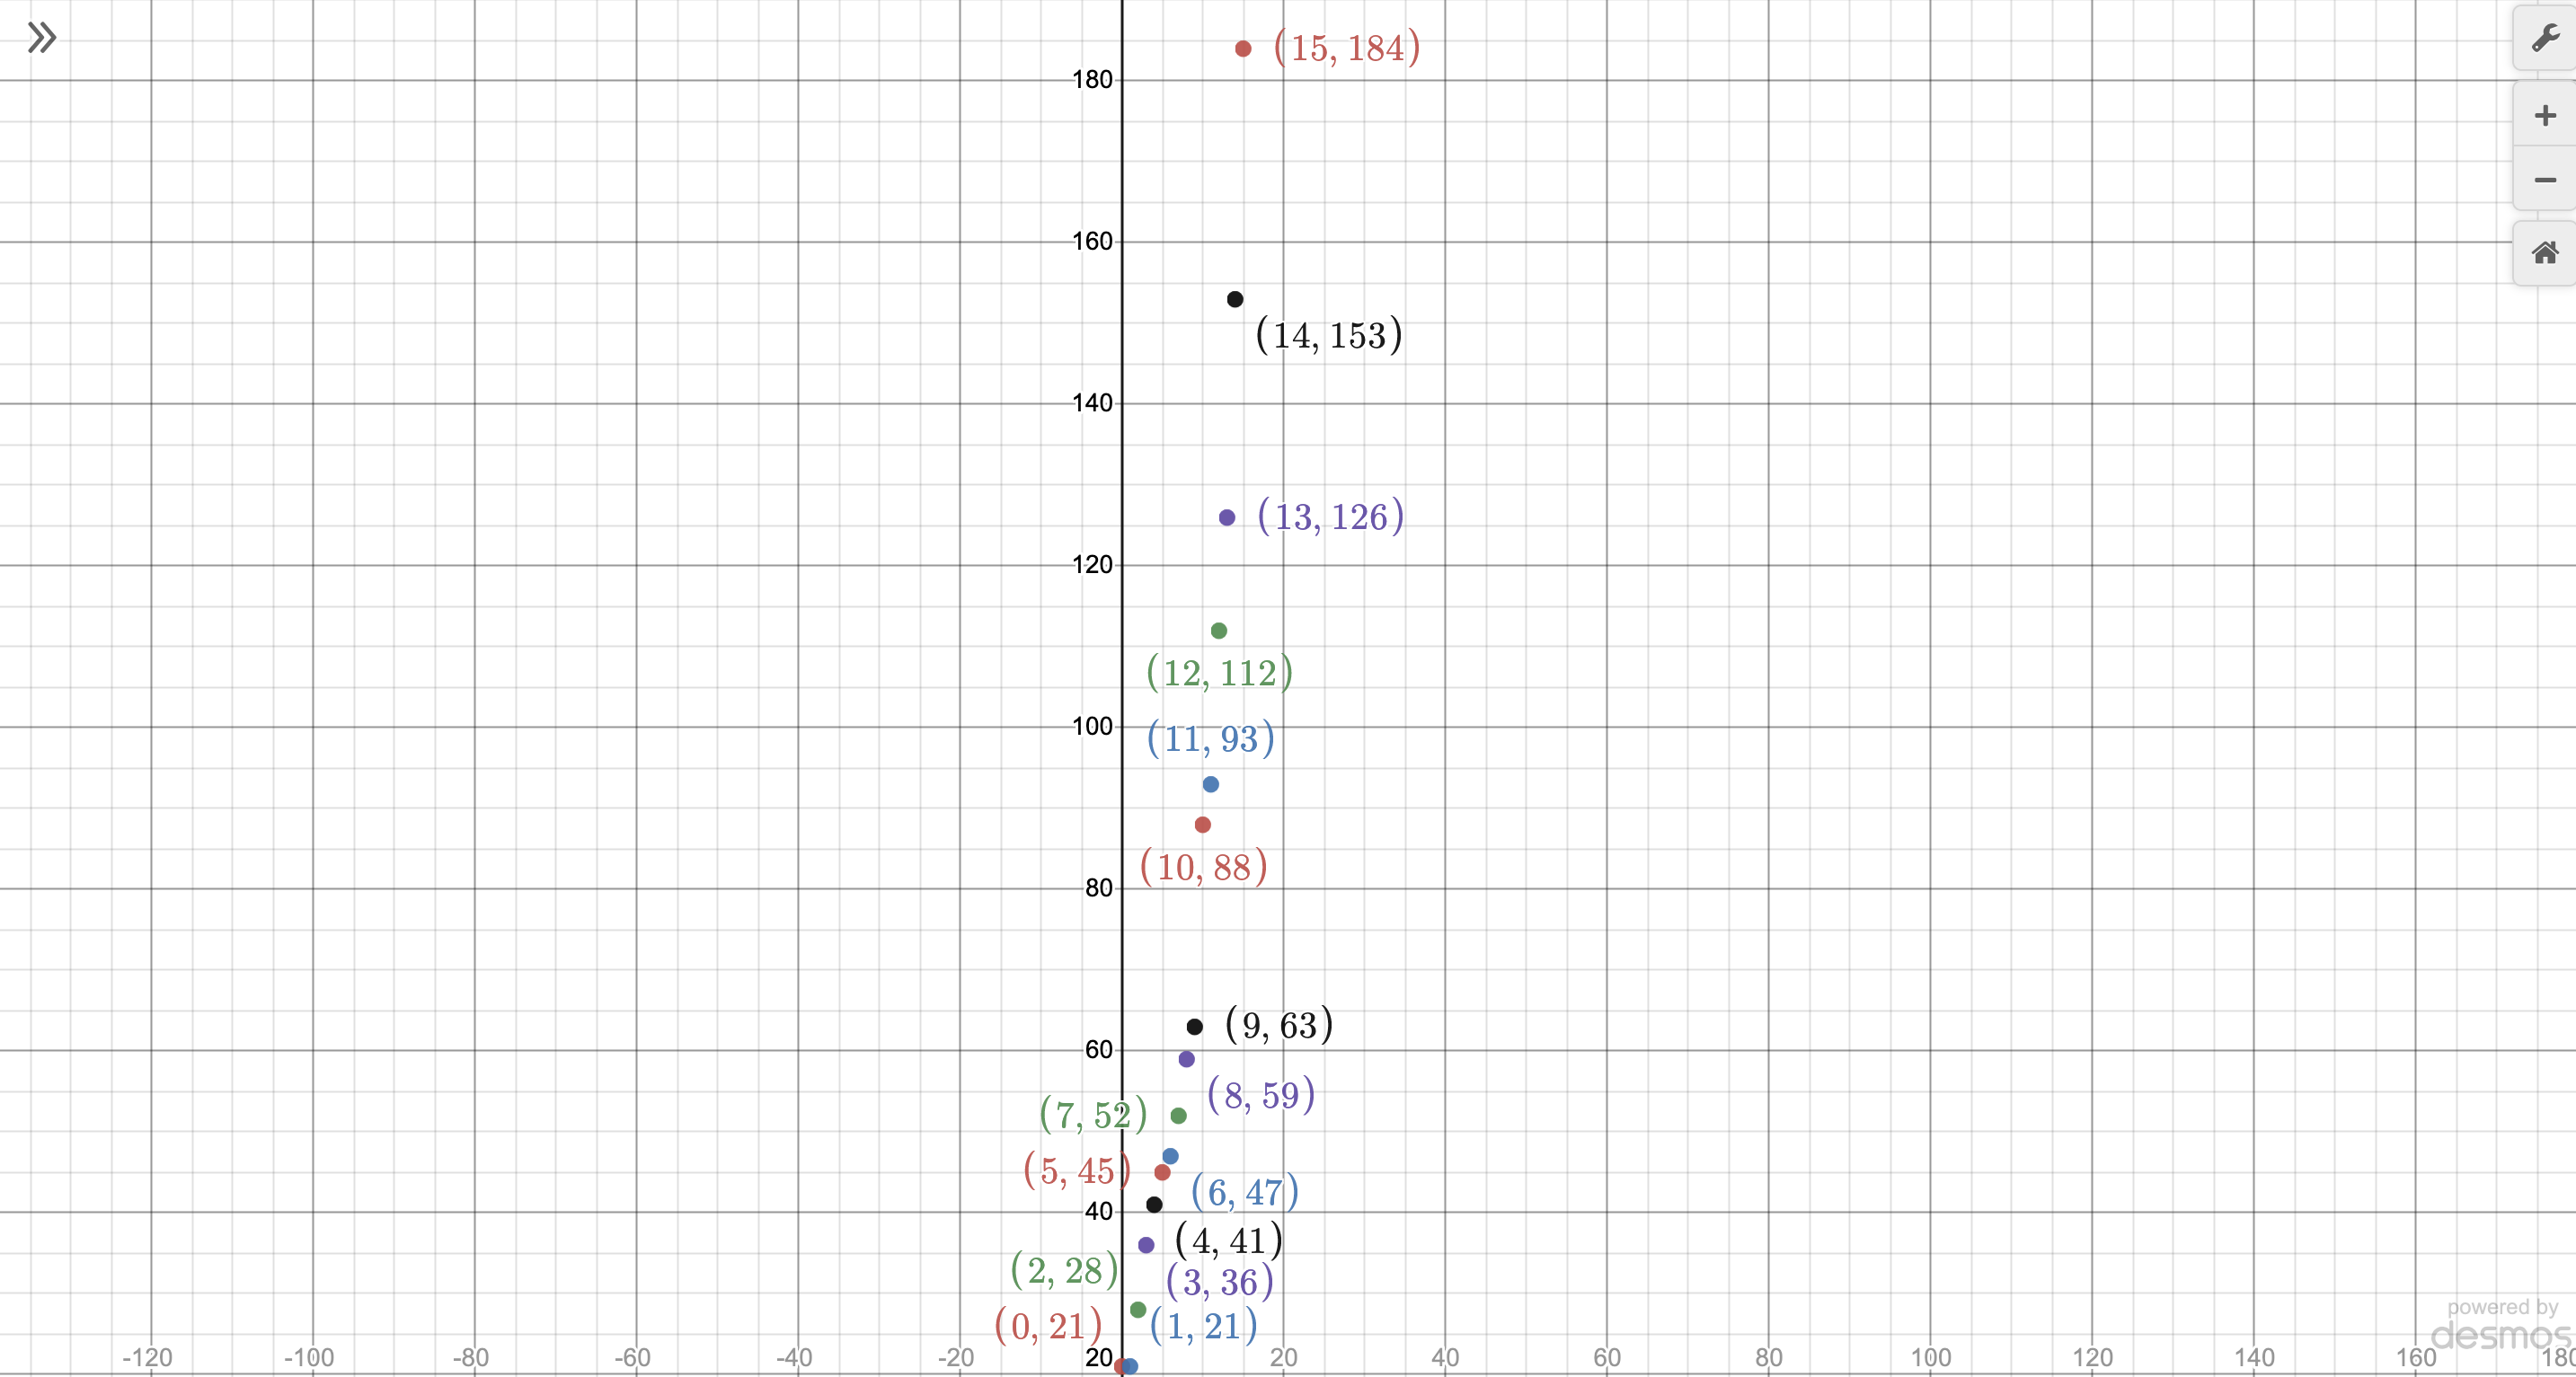
\includegraphics[width = 4in, height = 4in]{standard_testpicture1}
\newline
(b):\newline 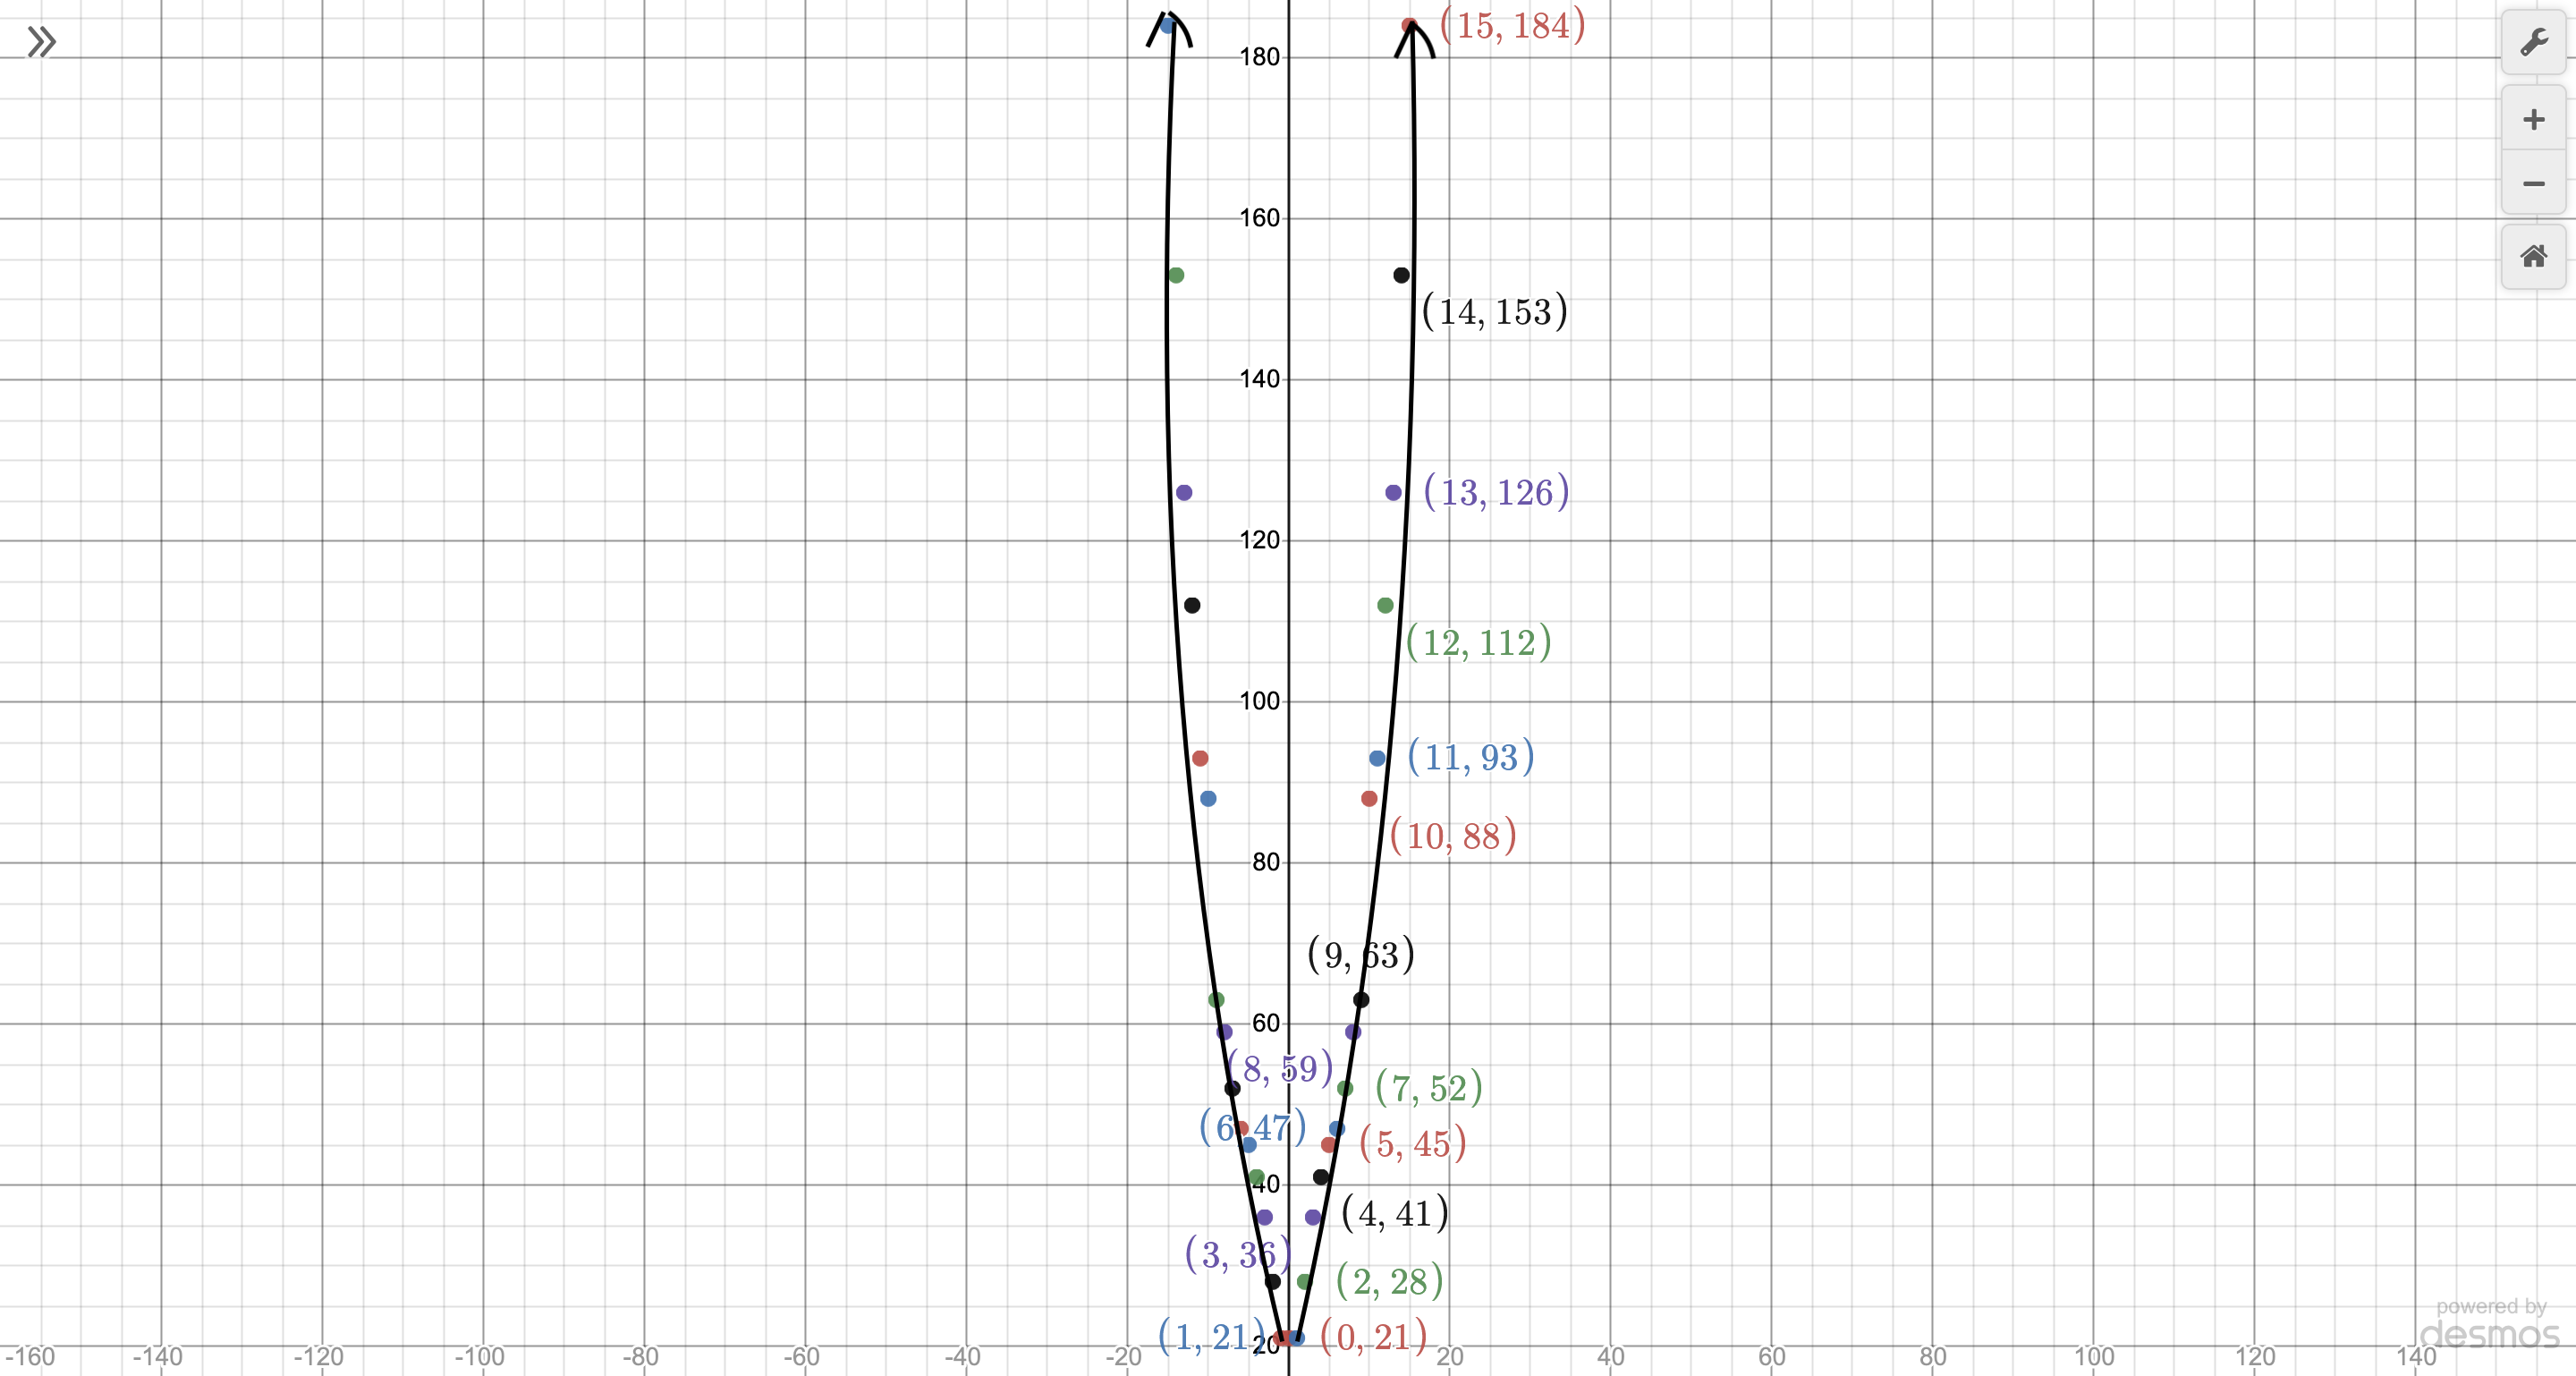
\includegraphics[width = 4in, height = 4in]{standard_testpicture2}
\newline
(c): First, as one can see on the graph, the vertex has an $x$-coordiante of $0.5$. I will estimate that the $y$-coordinate of the vertex is $20$ In 
addition, from looking at the graph, it seems that $(7.5,55)$ is close to being a point on the parabola, so I will also estimate that $(7.5,55)$ and 
$(-7.5,55)$ are also points on the graph. With this information, we can write the equation in vertex form: $y=a(x-0.5)^2+20$. Then, plugging in 
the second point estimated, we can solve for $a$:\newline 
$55=a(7.5-0.5)^2+20\newline\rightarrow 
49a=35\newline\rightarrow 
a=\frac{5}{7}$\newline meaning the model for the parabola is $y=\frac{5}{7}(x-0.5)^2+20$\newline
(d): \newline
\FloatBarrier
\begin{table}[h!]
        \begin{center}
                \begin{tabular}{l|c|c|c|c|c|c|c|r}
                        $Years\ since\ 1989$ & $0$ & $1$ & $2$ & $3$ & $4$ & $5$ & $6$ & $7$\\
                        \hline
                        $Payroll$ & $20.2$ & $20.2$ & $21.6$ & $24.5$ & $28.8$ & $34.5$ & $41.6$ & $50.2$
                \end{tabular}
        \end{center}
\end{table}

\begin{table}[h!]
        \begin{center}
                \begin{tabular}{l|c|c|c|c|c|c|c|r}
                        $Years\ since\ 1989$ & $8$ & $9$ & $10$ & $11$ & $12$ & $13$ & $14$ & $15$\\
                        \hline
                        $Payroll$ & $60.2$ & $71.6$ & $84.5$ & $98.8$ & $114.5$ & $131.6$ & $150.2$ & $170.2$
                \end{tabular}
        \end{center}
\end{table}
\FloatBarrier
From the above tables, it can be seen that there are no values that are shared between the model 
and the acutal table. However, most of the values from the model and the actual values are within a range 
of $5$. This means that while the model is certainly not accurate, it could be used potentially to make 
a rough estimate of the values of the payroll for each year.

\section*{22}
(a): The $x$-coordinate of the vertex of any standard form quadratic function is given by $-\frac{b}{2a}$. In addition, substituting this value in for 
$x$, when $a<0$, gives the $maximum\ value$. The maximum height is just another way of saying the maximum value (probably when $y$ is measured in some 
measurement for height). Hence, the maximum height of the volley ball, because $a=-16<0$, can be found by plugging in $-\frac{30}{2(-16)}=\frac{15}{16}
$ into the given equation, that is:\newline 
$-16(\frac{15}{16})^2+30(\frac{15}{16})+6=\frac{321}{16}$\newline
(b): The time at which the volley ball reaches its maximum height is the $t$ for which $h$ is the maximum height. From part (a), we already know that 
this value of $t$ is $-\frac{b}{2a}$, or $\frac{15}{16}$.\newline
(c): To find when the volley ball hits the ground, we need to find the roots of the equation $-16t^2+30t+6=0$, as this tells us when the height of the 
volley ball is equal to $0$ feet, that is, on the ground. We can do this by using the quadratic formula:
\[
\begin{array}{rl}
            & -16t^2+30t+6=0 \\
\rightarrow & t=\frac{-30\pm\sqrt{30^2-4(-16)(6)}}{2(-16)} \\
\rightarrow & t=\frac{-30\pm\sqrt{1284}}{-32} \\
\rightarrow & t=\frac{30+\sqrt{1284}}{32}=\frac{15+\sqrt{321}}{16}\vee t=\frac{15-\sqrt{321}}{16}
\end{array}
\]
and taking the positive intercept (because it does not make sense 
for time to be negative in this situation), we get $t=\frac{15+\sqrt{321}}{16}\approx 2.06$, meaning the volleyball takes about $2.06$ seconds to hit 
the ground.
\end{document}
